\documentclass[11pt]{report}
\usepackage[margin=2.5cm]{geometry}
\usepackage[french]{babel}
\usepackage[T1]{fontenc}
\usepackage[explicit]{titlesec}
\usepackage{times}
\usepackage{hyperref}
\usepackage{fancyhdr}
\usepackage{graphicx}
\usepackage{ucs}
\usepackage[utf8x]{inputenc}
\usepackage{awesomebox}
\usepackage{fontawesome5}
\usepackage{minted}
\setmainfont{Liberation Serif}

\titleformat{\chapter}[display]{\Huge}{\thechapter. #1}{20pt}{\small}

\titlespacing{\chapter}{0pt}{.1cm}{.1cm}

\lhead[\rightmark]{\rightmark}
\chead[]{}
\rhead[\thepage]{\thepage}

\lfoot[]{}
\cfoot[\thepage]{\thepage}
\rfoot[]{}

\renewcommand{\headrulewidth}{0.5pt}

\pagestyle{fancy}

\begin{document}
\begin{titlepage}
   \begin{center}
       \vspace*{5cm}

       \Huge\textbf{Manuel utilisateur}

       \vspace{0.5cm}
       \Large


       Moteur 3D - 7Physics


       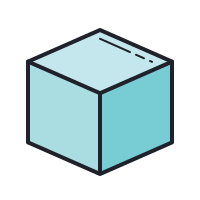
\includegraphics[width=2cm]{./logo.png}

       \vspace{1cm}

       \large
       \textbf{Équipe 3 : Noa AMMIRATI, Fanny DELNONDEDIEU, Quentin GENDARME, Pierre LOTTE, Théo PIROUELLE, Éléa TURC}

       \vfill

       
\includegraphics[width=15cm]{./enseeiht.jpeg}

       \vspace{2cm}

       ENSEEIHT\\
       Département Sciences du Numérique\\
       1APP SN 2020-2021


   \end{center}
\end{titlepage}


\tableofcontents

\chapter{Introduction}
L'objectif de ce manuel est de donner à l'utilisateur les bases nécessaires à la bonne utilisation de l'application.
L'application représente un moteur 3D permettant de réaliser des simulations de notions de physique élémentaires.
Un moteur 3D est un ensemble de fonctions permettant de représenter des objets dans un monde 3D, permettant de les
manipuler et de les afficher. Un autre objectif d'un moteur 3D est la gestion des interactions avec l'environnement (forces appliquées). \newline \newline


Les principales fonctionnalités du moteur 3D sont:
\begin{itemize}
        \item L'affichage de formes 3D prédéfinies et personnalisables (cube, sphere)
        \item L'utilisation de la caméra (permettant de changer d'angles de vue)
        \item L'animation des différentes formes contenues dans la scène 3D.
\end{itemize}

\chapter{Installation/Utilisation de l'application}

Pour pouvoir utiliser l'application, vous devez posséder Java8.
Voici comment installer cette version de Java :
\begin{itemize}
  \item Supprimer java de son système : sudo apt list --installed | grep jdk
  \item sudo apt remove (des résultats de la commande précèdente (ex: sudo apt remove openjdk-11-jdk))
  \item Installer java8 : sudo apt install openjdk-8-jdk
  \item Vérifier avec la commande : java -version\newline
\end{itemize}

Par la suite, pour exécuter le fichier .jar exécutable de l'application, il faut :
\begin{itemize}
  \item Pour Linux : java -jar file.jar
  \item Pour Windows : double-click sur le fichier
  \item Pour MacOS : java -jar file.jar\newline
\end{itemize}

\chapter{Présentation générale de l'application}

Voici l'interface de l'application :

\begin{figure}[h]
  \centering
  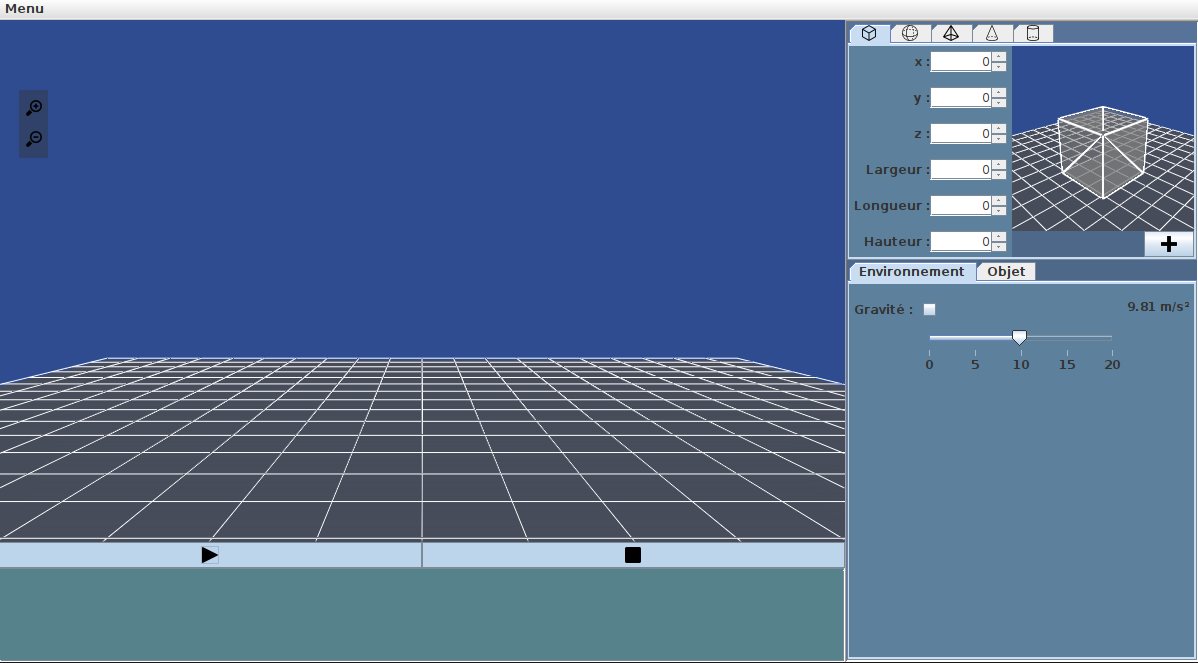
\includegraphics[scale=0.4]{./interface.png}
  \caption{Interface de l'application}
\end{figure}

L'application est structurée en 3 parties :
\begin{itemize}
  \item La partie centrale représente la scène 3D : c'est ici que l'utilisateur va visualiser
  les objets 3D ainsi que les intéractions.
  \item La partie située au-dessous de la scène 3D permet d'intéragir avec les objets en
  lançant une simulation (bouton play). Elle permet aussi d'afficher la liste des objets présents
  sur scène.
  \item La partie de droite permet de paramètrer la scène : ajout d'un cube, ajout d'une sphère,
  activation de la gravité, ajout de force sur les différents objets, suppresion d'un objet.\newline
\end{itemize}


Dans la suite de ce manuel, vous trouverez l'explication des différents fonctionnalités fournies
par l'application vous permettant alors la prise en main de celle-ci.


\chapter{Manipuler des objets 3D}

\section{Ajouter un objet 3D}
Pour pouvoir ajouter un objet 3D sur la scène 3D, il faut sur la partie supérieur droite de l'interface, sélectionner la forme souhaitée.
\newline

\notebox{Pour afficher un \textbf{cube} sur la scène 3D, il faut sélectionner le bouton : 
\includegraphics[width=0.4cm]{./btn_cube.png}
et remplir les informations demandées.\newline Pour afficher d'autres formes, il suffit de sélectionner les boutons adjacente.}

\begin{figure}[h]
  \centering
  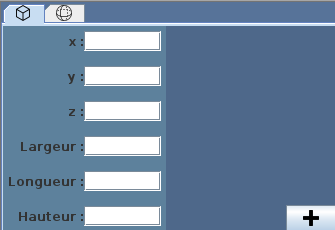
\includegraphics[scale=0.75]{./ajoutFormes.png}
  \caption{Ajout d'une forme}
\end{figure}

\section{Supprimer un objet 3D}

Afin de supprimer un objet 3D, il faut tout d'abord le sélectionner dans la partie inférieure de l'interface en cliquant sur un des boutons
présent. Une fois cela fait, rendez-vous dans l'onglet \flqq\ Objet \frqq en bas à droite de l'interface. Vous n'avez plus qu'à cliquer sur le
bouton supprimer : 
\includegraphics[width=1cm]{./btn_supprimer.png}.

\begin{figure}[h]
  \centering
  
\includegraphics{./supprimerForme.png}
  \caption{Suppression d'une forme}
\end{figure}

\chapter{Gestion de la caméra}

\warningbox{Afin de manipuler la caméra au clavier il est important de cliquer sur la scène en premier lieu. Sans cela, la caméra ne bougera pas.}

Afin d'observer la scène sous plusieurs angles, il est possible de manipuler la caméra. Les opérations possibles sont:
\begin{itemize}
        \item \hyperlink{zoom}{Zoomer}/\hyperlink{dezoom}{Dézoomer}
        \item \hyperlink{move}{Déplacements basiques (Gauche, droite, avant, arrière)}
        \item \hyperlink{moveV}{Se déplacer verticalement}
        \item \hyperlink{rotate}{Faire tourner la caméra.}
\end{itemize}

\section{Gestion du zoom}

Lors de la visualisation de la scène que vous avez créé, il vous est possible de régler le niveau de zoom utilisé afin de voir un objet plus en détail ou bien encore de voir une scène de taille importante en intégralité. Afin de réaliser ces actions, référez-vous aux explications suivantes.

\awesomebox{\faMousePointer}{3pt}{teal}{Attention, la gestion du zoom ne peut s'effectuer qu'à la souris.}

\subsection{Zoomer}

\hypertarget{zoom}{Il existe 2 possibilités pour zoomer sur la scène.}
\begin{itemize}
        \item La première est d'utiliser le bouton prévu à cet effet présent sur la gauche de votre écran représenté par ce symbole: 
\includegraphics[width=0.4cm]{./btn_zoom-in.png}.
        \item La seconde est d'utiliser la molette de votre souris en la faisant glisser vers le haut.
\end{itemize}

\subsection{Dezoomer}

\hypertarget{dezoom}{Il existe 2 possibilités pour dezoomer la scène.}

\begin{itemize}
        \item La première est d'utiliser le bouton prévu à cet effet présent sur la gauche de votre écran représenté par ce symbole: 
\includegraphics[width=0.4cm]{./btn_zoom-out.png}.
        \item La seconde est d'utiliser la molette de votre souris en la faisant glisser vers le bas.
\end{itemize}

\notebox{Afin de mieux maitriser votre environnement et de bénéficier d'une précision accrue, veuillez privilégier l'utilisation de la molette. En effet, les boutons latéraux sont limités à une manipulation prédéfinie du zoom et ne sont pas réglables.}


\section{Se déplacer sur la scène}

Afin de vous balader au sein de la scène pour visualiser celle-ci sous différents points de vue, il vous est possible de déplacer la caméra. Vous pourrez ainsi déplacer la caméra sur 3 axes différents que nous allons voir.

\awesomebox{\faKeyboard}{3pt}{teal}{Attention, les déplacememnts sur la scène ne peuvent être effectués que via le clavier et les raccourcis présentés.}

\subsection{Déplacements basiques}

\hypertarget{move}{Les premiers déplacement que nous allons voir sont les déplacements basiques gauche, droite, avant et arrière.} Ces déplacements se feront à l'aide des touches ZQSD du clavier.

\begin{itemize}
  \item \textbf{Z}: Avancer.
  \item \textbf{Q}: Se déplacer vers la gauche.
  \item \textbf{S}: Reculer.
  \item \textbf{D}: Se déplacer vers la droite.
\end{itemize}

\subsection{Déplacement vertical}

\hypertarget{moveV}{Ensuite, il peut être utile de bouger la caméra verticalement.} Pour cela, nous utiliserons les touches Espace et Shift.

\begin{itemize}
  \item \textbf{ESPACE}: Monter la caméra.
  \item \textbf{SHIFT}: Descendre la caméra.
\end{itemize}

\section{Tourner la caméra}

\hypertarget{rotate}{Enfin, pour finir, le dernier mouvement possible est la rotation de la caméra.} Pour cela, il suffit simplement de cliquer sur la scène 3D puis de glisser la souris vers l'endroit où vous souhaitez tourner la caméra en maintenant le clic de la souris.

\awesomebox{\faMousePointer}{3pt}{teal}{Attention, la rotation de la caméra ne peut se faire que via la souris.}

\chapter{Animer la scène 3D}

Une fois les objets ajoutés à la scène, il est possible de leur appliquer des forces personnalisées puis de lancer la simulation qui prendra
donc en compte ces forces pour déplacer les objets de la scène.

\section{Ajouter des forces}

La première étape est donc d'ajouter des forces. Pour cela, il est nécessaire de préselectionner la forme souhaitée dans la partie inférieure
de l'interface en cliquant sur un des boutons semblable au bouton vert de la figure suivante:

\begin{figure}[h]
  \centering
  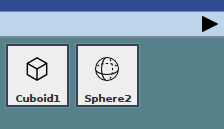
\includegraphics{./bouton_forme.png}
  \caption{Sélection d'une forme}
\end{figure}

Une fois la forme sélectionnée, la partie inférieure droite de l'interface, dans l'onglet \flqq\ Objet \frqq, sera mise à jour afin d'afficher
les informations liées à l'objet ajouté. Il est alors possible d'ajouter des forces en cliquant sur le bouton \textbf{+} disponible en haut
de la table intitulée \flqq\ Forces\frqq.

\begin{figure}[h]
  \centering
  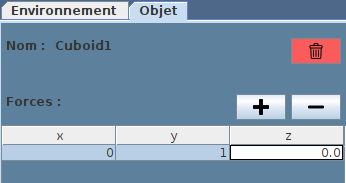
\includegraphics{./proprieteForme.png}
  \caption{Détails d'une forme}
\end{figure}

Une fois cela fait, et dès que vous changerez les valeurs de la ligne qui s'est ajoutée à la table, la force sera exercée sur l'objet.

\section{Supprimer des forces}

Afin de supprimer des forces, rendez-vous dans les détails de l'objet et cliquez sur la ligne contenant la force à supprimer. Une fois cela fait,
cliquez sur le bouton \textbf{-} de la table intitulée \flqq\ Forces \frqq.

\section{Lancer la simulation}

Afin de lancer la simulation, vous pouvez simplement appuyer sur le bouton Play disponible dans la partie inférieure de l'interface.

\begin{figure}[h]
  \centering
  
\includegraphics[width=16cm]{./btn_play.png}
  \caption{Lancement de la simulation}
\end{figure}

\section{Arrêter la simulation}

Afin d'arrêter la simulation, vous pouvez simplement appuyer sur le bouton Stop disponible dans la partie inférieure de l'interface.

\begin{figure}[h]
  \centering
  
\includegraphics[width=16cm]{./btn_stop.png}
  \caption{Arrêt de la simulation}
\end{figure}

\chapter{Importer et exporter un projet 3D}

Il est possible d'enregistre un projet 3D en cours sous forme d'un fichier pour le continuer plus tard à l'aide de
la fonctionnalité importer un projet 3D. Cet import peut aussi être fait à partir de fichiers créés par d'autre moteur 3D.

\section{Récupérer un projet 3D}

Pour importer un projet, il suffit d'ouvrir le menu déroulant en haut à gauche de l'écran et de sélectionner \flqq\ Importer un projet \frqq.
Une fenêtre de navigation de fichier s'ouvrira et vous pourrez ainsi choisir le fichier à importer.
Il est possible qu'une erreur apparaisse lors de l'importation pour cause d'une extension de fichier non valide (extension différente de \flqq\ .obj \frqq).

\begin{figure}[h]
  \centering
  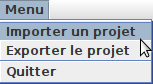
\includegraphics{./menu_imp.png}
  \caption{Sélection de l'importation sur le menu déroulant}
\end{figure}

\begin{figure}[h]
  \centering
  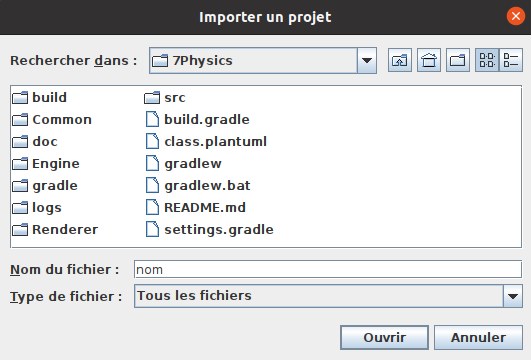
\includegraphics[scale=0.83]{./nav_fichier_imp.png}
  \caption{Navigateur de fichier permettant de sélectionner un fichier}
\end{figure}

\begin{figure}[h]
  \centering
  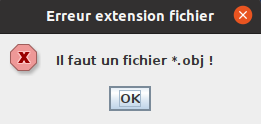
\includegraphics{./error_imp.png}
  \caption{Erreur lors de l'importation d'un fichier}
\end{figure}


\section{Sauvegarder un projet 3D}

De la meme manière, pour exporter la projet en cours et créer un fichier, on utilise le menu déroulant.
En sélectionnant \flqq\ Exporter un projet \frqq, une fenêtre s'ouvrira pour choisir l'emplacement et le nom du fichier à enregistrer.
Il est possible qu'une erreur apparaisse lors de l'exportation pour cause de la scène 3D vide.

\begin{figure}[h]
  \centering
  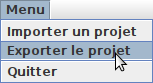
\includegraphics{./menu_exp.png}
  \caption{Sélection de l'exportation sur le menu déroulant}
\end{figure}

\begin{figure}[h]
  \centering
  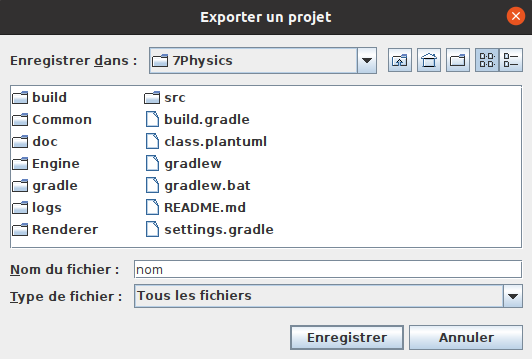
\includegraphics[scale=0.83]{./nav_fichier_exp.png}
  \caption{Navigateur de fichier permettant de sauvegarder un fichier}
\end{figure}

\begin{figure}[h]
  \centering
  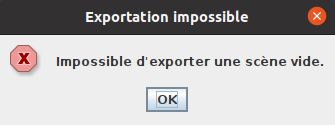
\includegraphics{./error_exp.png}
  \caption{Erreur lors de l'exportation d'un fichier}
\end{figure}

\chapter{Utilisation de l'API}

Pour utiliser les fonctionnalités de 7Physics il est nécessaire de tirer ses dépendances. Pour se faire il est nécessaire d'installer le plugin \href{https://jitpack.io/}{\color{blue}JitPack} à votre gestionnaire de dépendances.

Exemple avec gradle :

\begin{minted}{groovy}
repositories {
    mavenCentral()
    maven {
        url 'https://jitpack.io'
        metadataSources {
            artifact() //Look directly for artifact
        }
    }
}
\end{minted}

Vous pourrez ensuite ajouter les dépendances de 7Physics à votre projet :

\begin{minted}{groovy}
dependencies {
    implementation 'com.github.7Physics:Common:master-SNAPSHOT'
    // Si vous souhaitez utiliser le moteur de rendu :
    implementation group: 'org.jogamp.jogl', name: 'jogl-all-main', version: '2.3.2'
    implementation group: 'org.jogamp.gluegen', name: 'gluegen-rt-main', version: '2.3.2'
    implementation 'com.github.7Physics:Renderer:master-SNAPSHOT'
    // Si vous souhaitez utiliser le moteur physique :
    implementation 'com.github.7Physics:Engine:master-SNAPSHOT'
}
\end{minted}

\notebox{De part la façon dont a été structuré 7Physics il est possible d'utiliser le moteur de rendu avec un moteur physique différent, et inversement.}

Exemple d'utilisation :

\begin{minted}{java}
public static void main(String... args) {
    JFrame frame = new JFrame("Exemple 7Physics");

    Camera camera = new Camera(new Position(-3, 1, 0));
    camera.rotateVertical(-Math.PI/8);

    // On crée la scène 3D
    Scene3D scene = new Scene3D(camera);
    // C'est un panel comme les autres, on peut lui modifier ses dimensions et l'ajouter à un panel
    scene.setPreferredSize(new Dimension(1000, 600));
    frame.add(scene);

    frame.pack();

    frame.setDefaultCloseOperation(JFrame.EXIT_ON_CLOSE);
    frame.setVisible(true);

    // On crée le world qui contiendra les objets physiques
    World world = new World();
    world.setGravity(new Vec3(0, -1, 0));

    Position wallPosition = new Position(0, .15, -1);

    scene.addObject(new Cuboid(3, .1, 2))
         .setPosition(wallPosition);
    world.addPhysicObject(new Cuboid(3, 2, .1))
         .setPosition(wallPosition)
         .setDynamic(false);

    Random r = new Random();
    r.nextFloat();

    for(int i = 0; i < 100; i++) {
        // Position partagée entre l'objet graphique et l'objet physique : fait le lien entre eux.
        Position spherePosition = new Position(r.nextFloat()*6-3, (i+2)/3f, r.nextFloat()*6-3);

        // On ajoute la sphère graphique
        scene.addObject(new Sphere(.1, 3))
             .setPosition(spherePosition)
             .setColor(Color.ORANGE, Color.RED);
        // On ajoute la sphère physique
        world.addPhysicObject(new Sphere(.1, 3))
             .setPosition(spherePosition)
             .addForce(new Vec3(r.nextFloat()*4-2, 0, r.nextFloat()*4-2));
    }

    // On lance la simulation à 60 mise à jour par seconde
    world.startStepLoop(60);
}

\end{minted}

Résultat :

\begin{figure}[h]
  \centering
  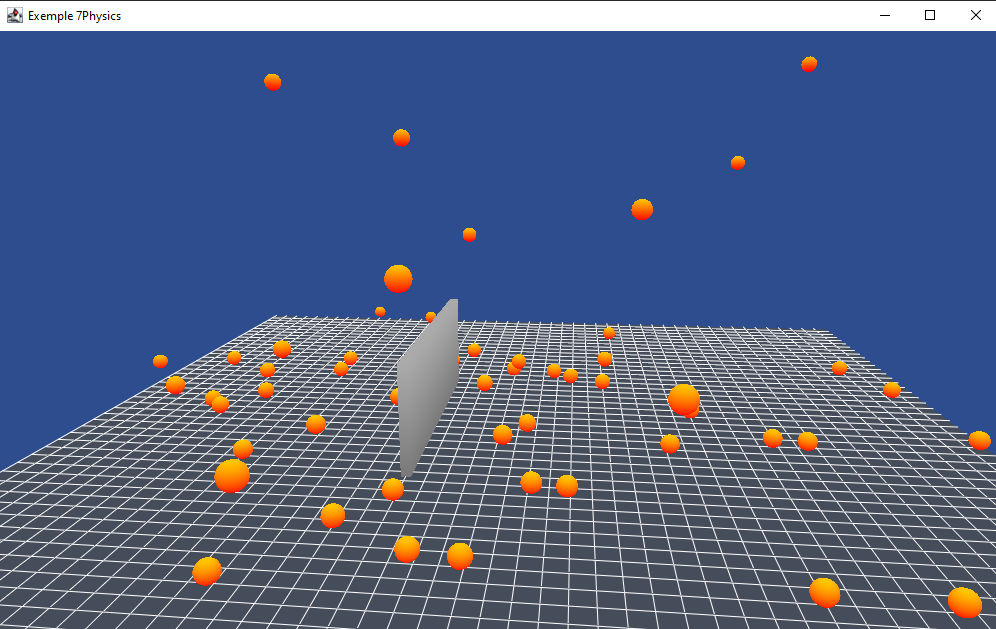
\includegraphics{./example.png}
  \caption{Rendu obtenu à partir du code précédent}
\end{figure}

\end{document}
